\section{Supplementary Material}

\begin{supplement}



\subsection{Digging into code}

%===============================================================================
\begin{figure}[h]
    \centering
    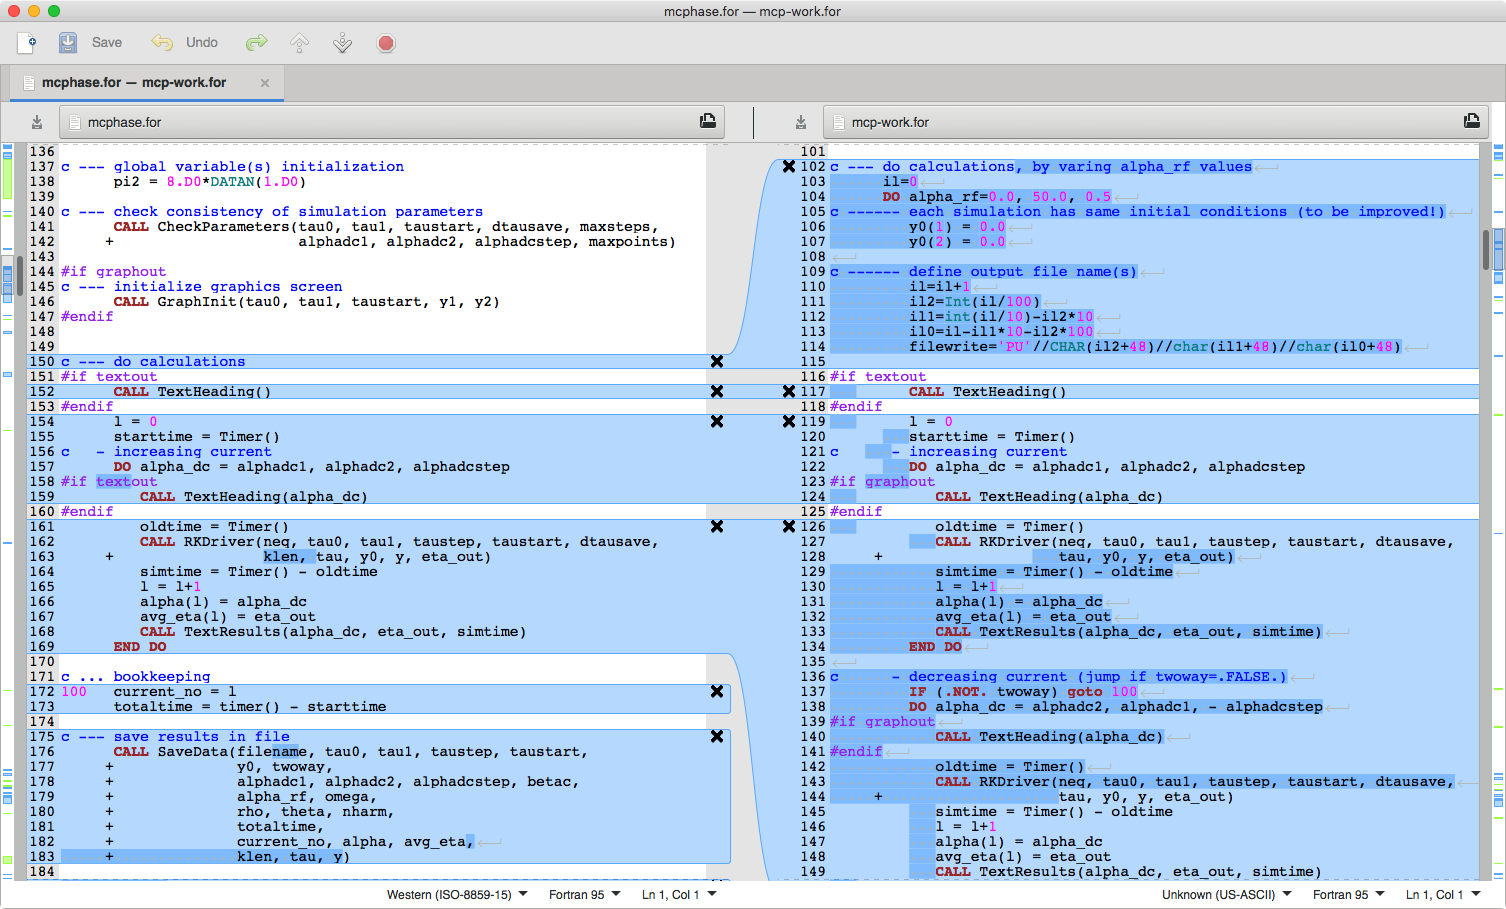
\includegraphics[width = 0.75 \textwidth]{meld-comparison.png}
    \caption{Comparison with Meld of the main calculation loop of (left) \textsf{mcphase.for} and (right) \textsf{mcp-work.for}.}
    \label{fig:meld-comparison}
\end{figure}
%===============================================================================

%===============================================================================
\begin{figure}[h]
    \centering
    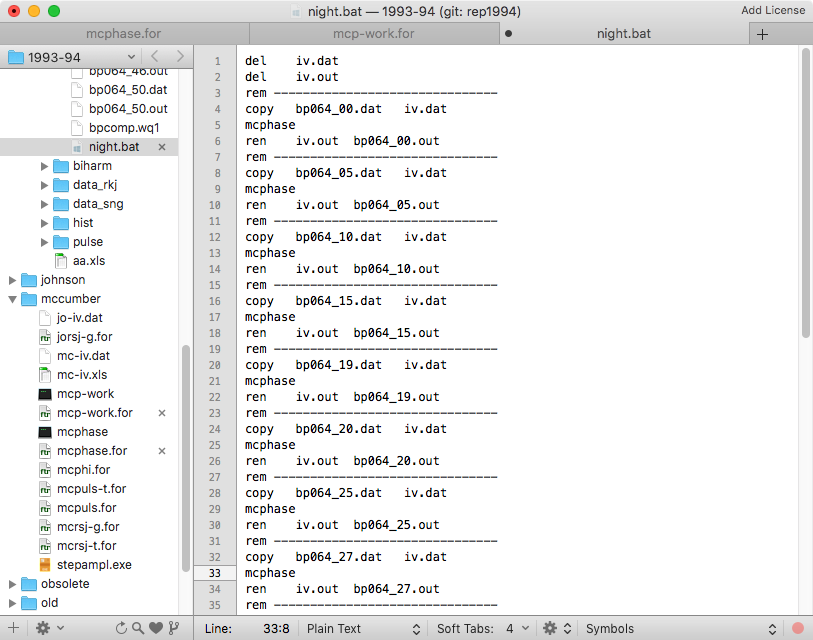
\includegraphics[width = 0.75 \textwidth]{batch-file.png}
    \caption{DOS batch file used by \textsf{mcphase.for} to run multiple simulations with different values of the amplitude of the microwave signal $\alpha_\mathrm{rf}$.}
    \label{fig:batch-file}
\end{figure}
%===============================================================================



\clearpage
\subsection{Preprocessor directives}

%===============================================================================
\lstset{
    language = C,
    basicstyle = \tiny\bfseries\ttfamily,
    tabsize = 4,
    frame = lines,
    framesep = 1em,
    framexleftmargin = 1em,
    backgroundcolor = \color{ultralightgray},
    keywordstyle = \color{darkred}\bfseries,
    morekeywords = {$DEFINE, $if, $endif, defined},
    deletekeywords = {for}
}
%===============================================================================
\begin{figure}[h]
\centering

\begin{minipage}{0.75\textwidth}
\textbf{(a)}
\begin{lstlisting}
      $DEFINE textout			! DEFINEd for text output
      c $DEFINE graphout		! DEFINEd for graphical output
      
      c $DEFINE single        ! DEFINED for single rf drive
      c $DEFINE biharmonic    ! DEFINED for biharmonic drive
      $DEFINE pulsed			! DEFINED for pulsed drive
      ...
      ...
      $if defined (graphout)
      	...
      $endif
      ...
      ...
      $if defined (textout)
      	...
      $endif
      ...
      ...
      $if defined (pulsed)
      	...
      $endif
      ...

\end{lstlisting}
\end{minipage}
%
\hfill
%
\begin{minipage}{0.75\textwidth}
\textbf{(b)}
\begin{lstlisting}
      CC $DEFINE textout		! DEFINEd for text output
      c $DEFINE graphout		! DEFINEd for graphical output
      
      c $DEFINE single        ! DEFINED for single rf drive
      c $DEFINE biharmonic    ! DEFINED for biharmonic drive
      CC $DEFINE pulsed		! DEFINED for pulsed drive
      ...
      ...
      #if graphout
      	...
      #endif
      ...
      ...
      #if textout
      	...
      #endif
      ...
      ...
      #if pulsed
      	...
      #endif
      ...

\end{lstlisting}
\end{minipage}

\caption{Preprocessor directives in (a) Microsoft Fortran 5.1, (b) modern \textsf{cpp} preprocessor.}
\label{fig:preprocessor}
\end{figure}
%===============================================================================



\clearpage
\subsection{Porting Microsoft Fortran to modern Unix}

%===============================================================================
\lstset{
    language = Fortran,
    basicstyle = \tiny\bfseries\ttfamily,
    tabsize = 6,
    frame = lines,
    framesep = 2em,
    framexleftmargin = 1em,
    backgroundcolor = \color{ultralightgray},
    keywordstyle = \color{darkred}\bfseries,
    morekeywords = {},
    deletekeywords = {}
}
%===============================================================================
\begin{figure}[h]
\centering

\begin{minipage}{0.75\textwidth}
\textbf{(a)}

\begin{lstlisting}
    ...
    INTEGER*2      iyr, imon, iday
    INTEGER*2      ihr, imin, isec, dummy
    ...
    ...
    CALL GETDAT(iyr, imon, iday)
    CALL GETTIM(ihr, imin, isec, dummy)
    ...

\end{lstlisting}
\end{minipage}
%
\hfill
%
\begin{minipage}{0.75\textwidth}
\textbf{(b)}
\begin{lstlisting}
      ...
      character*8    date
      character*10   time
      character*5    zone
      integer        values(8)
      ...
      ...
      call date_and_time(date, time, zone, values)
      ...
      ...
      iyr  = values(1)
      imon = values(2)
      iday = values(3)
      ihr  = values(5)
      imin = values(6)
      isec = values(7)
      ...

\end{lstlisting}
\end{minipage}

\caption{Getting the date and time in (a) Microsoft Fortran 5.1, (b) modern gfortan.}
\label{fig:date-time}
\end{figure}


\end{supplement}

